\section{Trigger link}
The trigger link is a connection between the optical serial link board (oSLB) in the HCAL trigger and readout cards (HTR) of the HO system in the service cavern to the TwinMux. This link provides trigger data from all HO tiles that are matched to the towers of the rest of the calorimeter system.\\
With this trigger link, which is used to create a technical trigger, the impact of HO information on the L1 trigger rate and the minimal required granularity for ghost busting purposes can be determined.
The different components and the setup and idea for a data format are explained in the next sections.
\subsection{Setup}
The trigger link includes the TwinMux and the HTR withtin the HO system. The relevant parts of the system are explained.
\subsubsection{TwinMux}
The TwinMux is an FPGA based device that receives trigger data from RPC, DT and HO and can be programmed to merge this information to output trigger information using all three sub-detectors in CMS. With the current design the TwinMux can handle up to seven optical input cables coming from HO. The aim is to use only three inputs for HO as maximum.
\subsubsection{HTR and HO setup}
The general HTR and HO setup is shown in figure \ref{HOPlan}.\\
\begin{figure}[b]
\centering
\begin{minipage}[t]{0.95\textwidth}
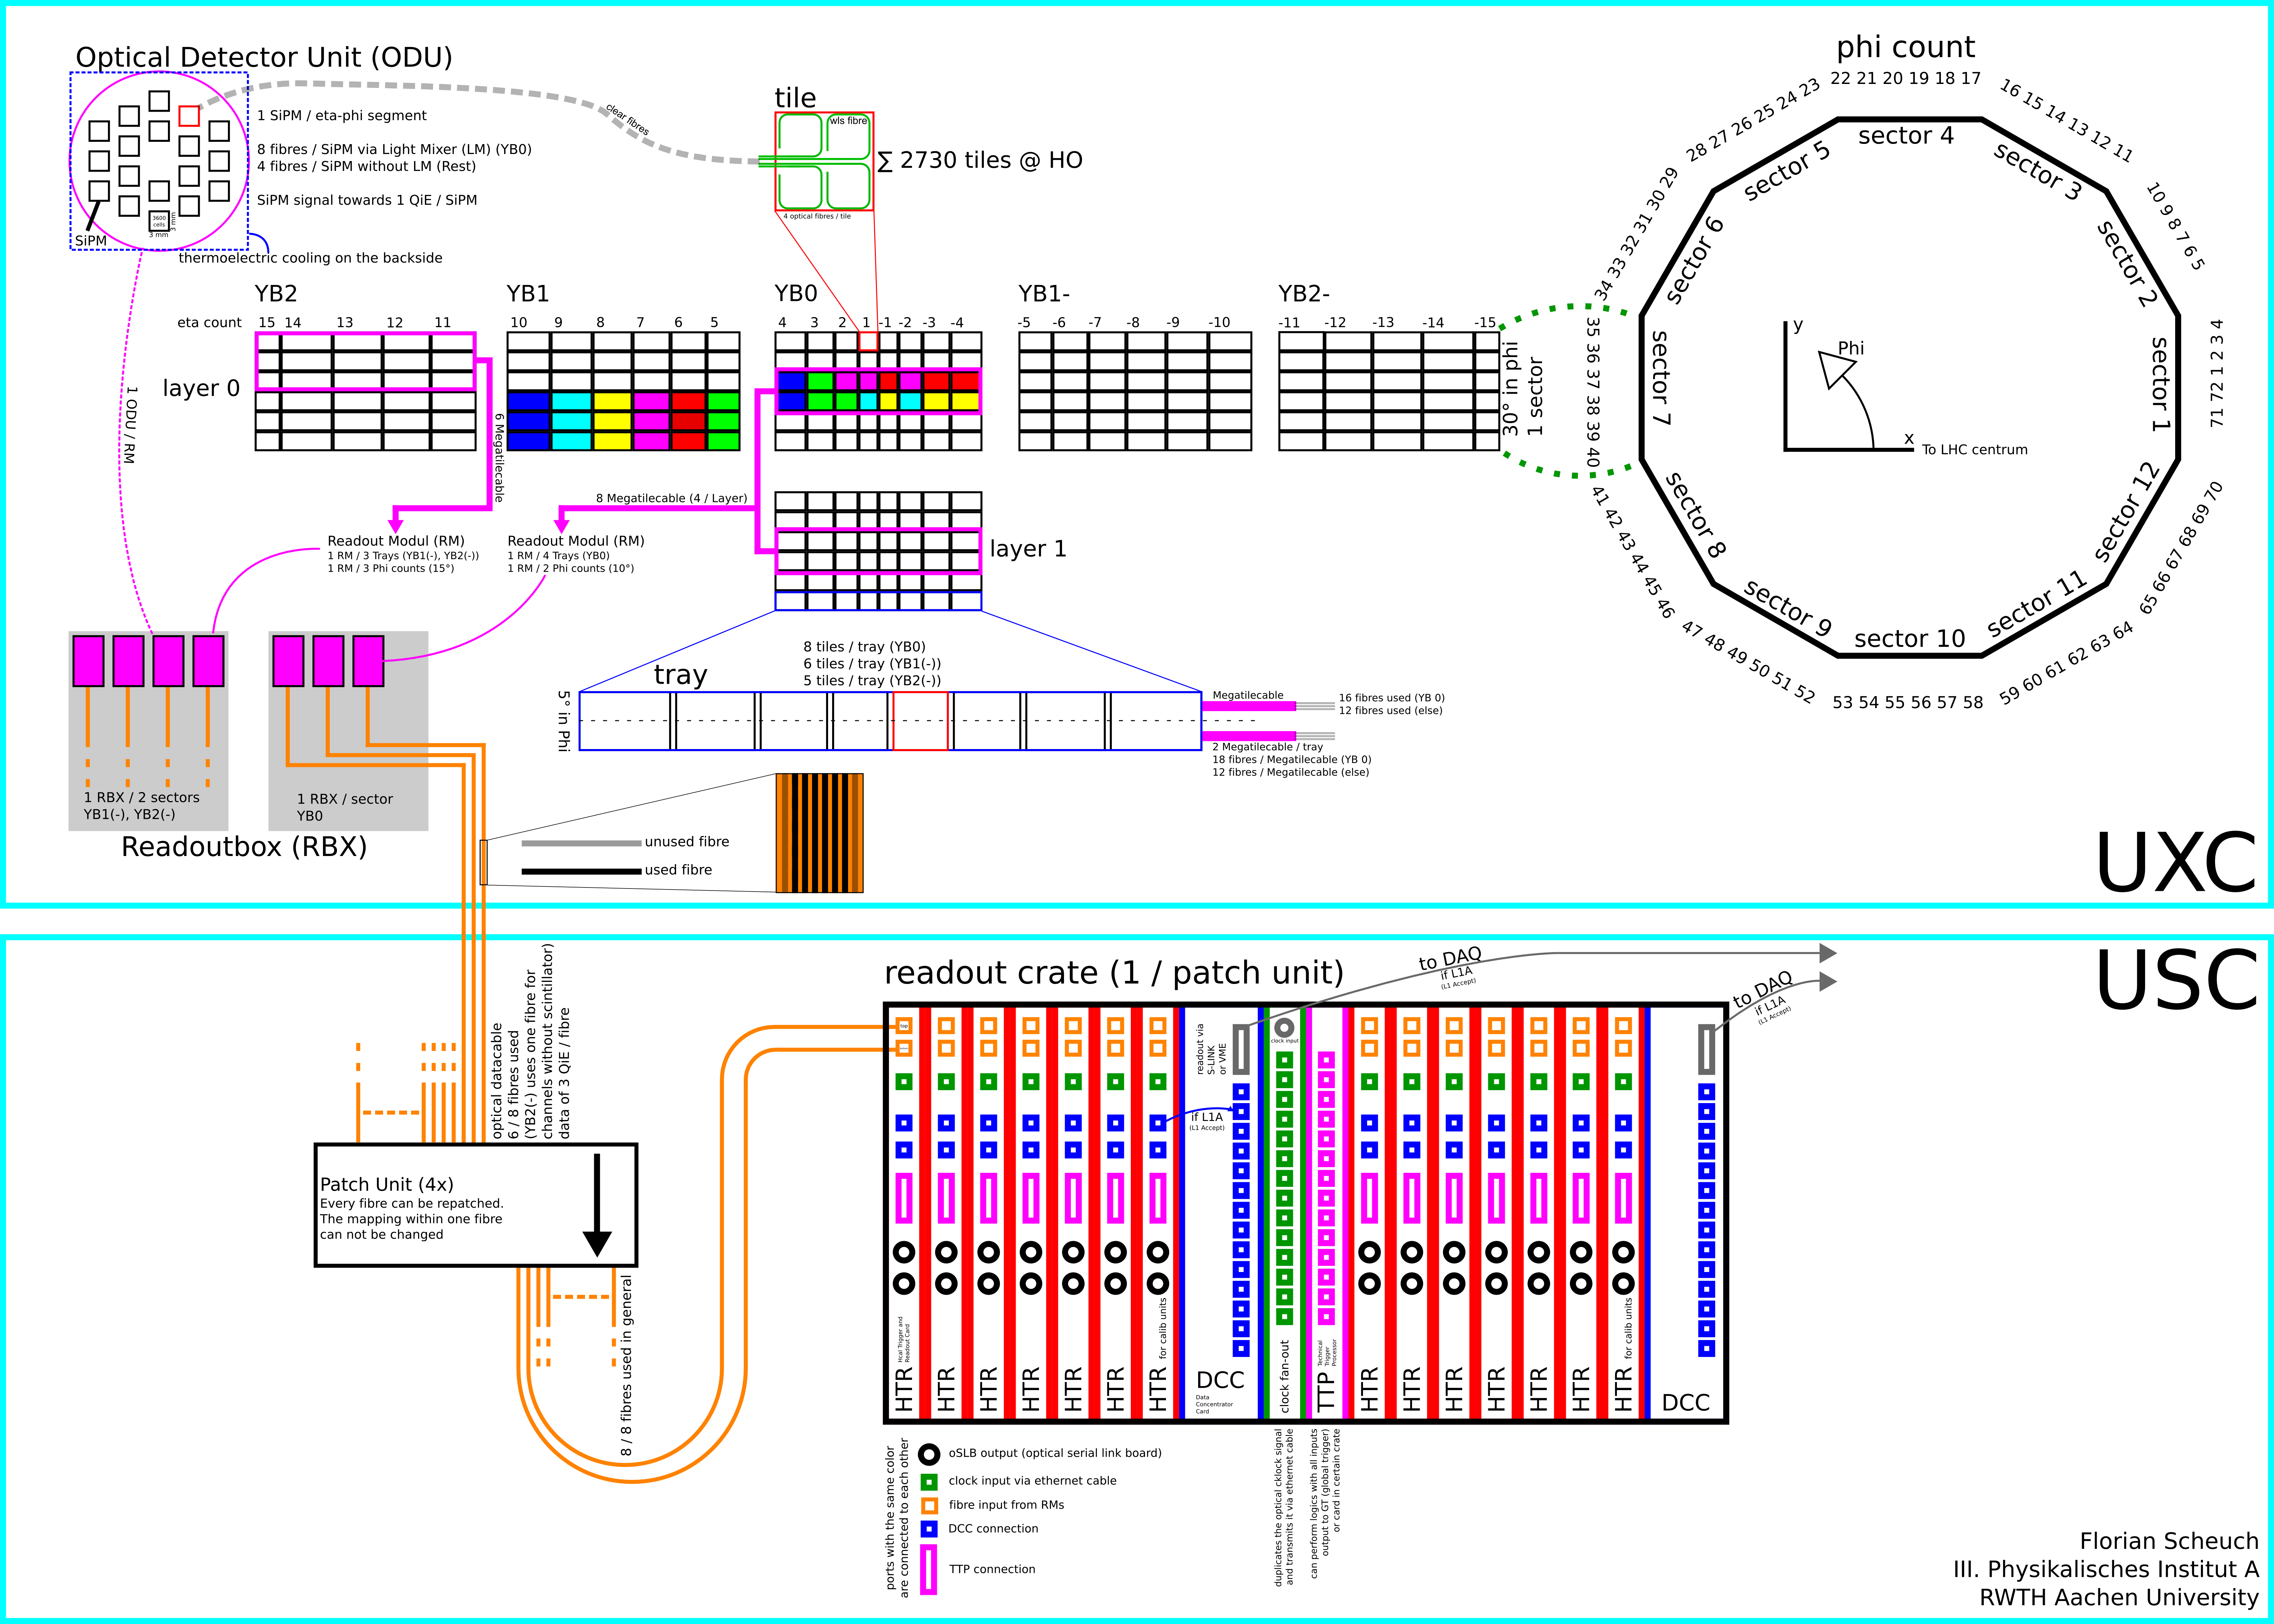
\includegraphics[height=\textwidth, angle=90]{Figures/scheuch/Chart.png}
\caption{Draft of the HO setup in USX and USC}
\label{HOPlan}
\end{minipage}
\end{figure}
Each HO tower signal is detected by one SiPM. An SiPM is placed with 17 other SiPMs on an optical detector unit (ODU). An ODU is placed on a readout module (RM). Three readout modules in YB0 and four RM in YB1(-),YB2(-) are located on a readout box (RBX). In YB0 an RBX collects the information of one sector. In YB1(-) and YB2(-) an RBX collects the information of 2 sectors.\\
Every RM has an optical cable as output. Each cable has 8 fibers which can transmit the data of three SiPM each. Only 6 of these 8 fibers are used.\\
All optical cables lead to the service cavern where the fibers can be patched. The information within a fiber can not be patched. After the patching, all 8 fibers within a cable are used and directed to the HCAL readout and trigger cards (HTR).\\
The HTRs are located in the HO crates in the service cavern. Each crate contains 14 HTR of which 2 are for calibration purposes. Each HTR receives the digitized energy information of 2*24 = 48 HO tiles per time slice (25 ns). Two FPGAs process the data of 24 HO tiles, each. If the energy in three adjacent time slices exceeds a certain threshold, the trigger bit for this particular channel is set true for the respective bunch-crossing (BX).
Each HTR FPGA sends 36 bits/BX to the oSLB. These 36 bits contain 24 bits of muon data, 8 bits bunch crossing number, 1 bit bunch crossing zero and 3 bits are not used.
\subsubsection{oSLB}
The optical serial link board (oSLB) is the interface of a HTR card to transmit data from the FPGA optically to any capable receiver. (In this case the receiver is the TwinMux.) It was installed in 2008 in the USC. Each HTR has three oSLB outputs of which every output can send 32 bits/BX. The 32 bits can contain up to 24 trigger bits. The remaining 8 bits are reserved for bunch-crossing ID and a check sum. Constrained by the number of three outputs, the internal HO mapping has to be chosen that the information processed in a HTR is relevant for three TwinMux maximum.
\subsubsection{Prerequisites for the trigger link}
Currently, optical cables are wired from the oSLBs to the RPC. To establish the trigger link on the hardware side of HO, the cables have to be plugged into the oSLBs and into the TwinMux. Furthermore, the TwinMux is currently designed and prototypes are build. With these prototypes a firmware is written to handle the incoming data.\\
The mapping of the different HO tiles has to be rerouted, such that every HTR card has only information that goes to three different TwinMux at maximum. This is due to the fact that every HTR has only three oSLB outputs.\\
Therefore, this mapping has to be clear and must be programmed into the oSLB firmare. Currently, the oSLB firmware is examined. As a second prerequisite, the interface between oSLB and TwinMux has to be clear in terms of data formats. A discussion between the TwinMux group and the responsibles for oSLB is ongoing. As soon as this information is available the oSLB firmware can be written.\\
To write the oSLB firmware, a HTR card including oSLB is nescessary. These devices are present at DESY.